\chapter{Introducció}

El problema a resoldre consisteix en trobar un impuls $\Delta V$ inicial que porti una nau d'un planeta a un altre, donats els instants de sortida $t_1$ i d'arribada $t_2$, i els planetes d'origen i destí.

Per tal de fer això, primer s'han de trobar els elements orbitals eclíptics de l'òrbita de transferència d'un planeta a l'altre així com les velocitats heliocèntriques de sortida i d'arribada de la sonda als respectius planetes. Finalment, a partir d'aquestes velocitats, es pot obtenir el $\Delta V$ i determinar així la viabilitat del viatge.

Es tracta d'un projecte complex que toca gran part del contingut vist a la part de mecànica orbital de l'assignatura \textit{Aerodinàmica, Mecànica de Vol i Mecànica Orbital} del Màster d'Enginyeria Aeronàutica de l'UPC. Per aquest motiu, ha despertat l'interès de l'equip i ha sigut l'escollit.

\section{\textit{Patched Conics Approximation}}
La metodologia matemàtica que s'ha seguit consisteix en el mètode de \textit{Patched Conics Approximation} \cite{Calaf2017d}. Segons aquest, la trajectòria es divideix per zones d'influència. És a dir, en un problema exacte, caldria tenir en compte la influència del Sol i de tots els objectes del Sistema Solar en cada moment. Tanmateix, en aquest mètode es suposa que cada planeta té una esfera d'influència (EdI) dins de la cual un cos només es veu atret per la força gravitatòria que exerceix aquest planeta. Fora de l'EdI, s'assumeix que l'única força gravitatòria és la que fa el Sol. Aquesta esfera d'influència depèn de la distància entre els cossos que exerceixen la força gravitatòria i de la seva massa segons l'expressió:
\begin{equation}
R_{I}=R\left(\frac{m_{planeta}}{m_\odot}\right)
\end{equation}
En aquest cas, ja que ens trobem dins del Sistema Solar, $R$ és la distància del planeta al Sol, $m_\odot$ la massa del Sol, $m_{planeta}$ la massa del planeta i $R_{I}$ la seva esfera d'influència.

Així, en un viatge interplanetari, inicialment la sonda es troba dins de l'esfera d'influència del planeta de sortida. Un cop surt d'aquesta, està només sota la influència del Sol. I en arribar al planeta de destí, està dins de la seva EdI. El mètode es basa en tenir sempre un problema de dos cossos, variant el cos central segons l'EdI, bé sigui un dels planetes o bé el Sol. D'aquesta forma es simplifica molt el problema. Per aquest motiu la \textit{PCA} va molt bé per càlculs inicials, tot i que s'hauran de refinar numèricament a posteriori si es volen resultats més precisos.

\section{Viatges interplanetaris}
Com s'ha resumit a l'apartat anterior, en el càlcul de la trajectòria interplanetària que segueix la sonda, es suposa sempre que es troba sota la influència d'un sol cos, ja sigui un planeta o el Sol. Tanmateix, la seva trajectòria serà diferent en funció de sota la influència de quin cos es trobi, com es pot veure a la Figura \ref{patchedconics}

\begin{figure}[H]
	\centering
	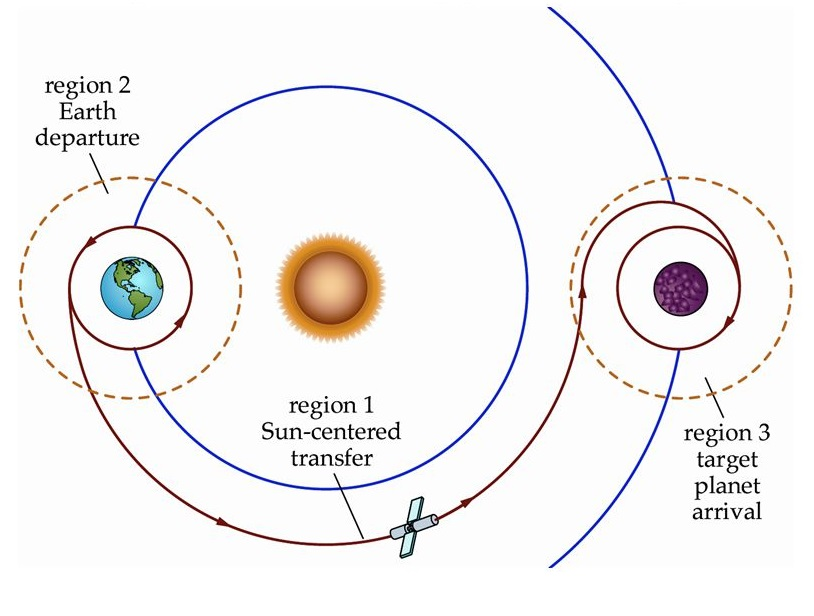
\includegraphics[scale=0.5]{./plots/patchedconics}
	\caption{Trajectòria interplatenària d'una nau utilitzant el mètode \textit{Patched Conics Approximation}}
	\label{patchedconics}
\end{figure}

Per tant, la trajectòria que seguirà el planeta es divideix en les següents fases:
\begin{enumerate}
	\item Sortida: El planeta es troba en una òrbita d'aparcament a sobre del planeta de sortida. Evidentment, aquesta òrbita es troba dins de l'esfera d'influència del planeta. És aquí on se li aplica el $\Delta V$ inicial en l'instant $t_{1}$. Un cop se li ha aplicat aquest impuls, la sonda segueix una trajectòria hiperbòlica que l'envia fora de l'esfera d'influència del planeta.
	\item Trajectòria interplanetària: Un cop ha sortit de l'esfera d'influència del planeta, la sonda es troba sota la influència únicament del Sol. En aquest moment fa l'òrbita de transferència de l'EdI del planeta d'origen a l'EdI del planeta de destí. Aquesta trajectòria pot ser el·líptica o hiperbòlica en funció dels temps de sortida i arribada dels planetes.
	\item Arribada: Un cop arriba a l'EdI del planeta de destí en l'instant $t_{2}$, la sonda deixa d'estar sota la influència del Sol i només és atreta pel planeta de destí. Un cop ha entrat en aquesta esfera d'influència segueix una trajectòria hiperbòlica. En funció de la hipèrbola, la sonda xocarà contra el planeta o el passarà de llarg. En aquest punt, si es vol que la sonda quedi orbitant el planeta caldrà aplicar-li un altre $\Delta V$.
\end{enumerate}